%%%%%%%%%%%%%%%%%%%%%%%%%%%%%%%%%%%%%%%%%
% Dreuw & Deselaer's Poster
% LaTeX Template
% Version 1.0 (11/04/13)
%
% Created by:
% Philippe Dreuw and Thomas Deselaers
% http://www-i6.informatik.rwth-aachen.de/~dreuw/latexbeamerposter.php
%
% This template has been downloaded from:
% http://www.LaTeXTemplates.com
%
% License:
% CC BY-NC-SA 3.0 (http://creativecommons.org/licenses/by-nc-sa/3.0/)
%
%%%%%%%%%%%%%%%%%%%%%%%%%%%%%%%%%%%%%%%%%

%----------------------------------------------------------------------------------------
%	PACKAGES AND OTHER DOCUMENT CONFIGURATIONS
%----------------------------------------------------------------------------------------

\documentclass[final,hyperref={pdfpagelabels=false}]{beamer}

\usepackage[orientation=portrait,size=a1,scale=1.4]{beamerposter} % Use the beamerposter package for laying out the poster with a portrait orientation and an a0 paper size

\usetheme{I6pd2} % Use the I6pd2 theme supplied with this template

\usepackage[english]{babel} % English language/hyphenation

\usepackage{amsmath,amsthm,amssymb,latexsym} % For including math equations, theorems, symbols, etc
\usepackage{bbm}

%\usepackage{times}\usefonttheme{professionalfonts}  % Uncomment to use Times as the main font
%\usefonttheme[onlymath]{serif} % Uncomment to use a Serif font within math environments

\boldmath % Use bold for everything within the math environment

\usepackage{booktabs} % Top and bottom rules for tables

\graphicspath{{figures/}} % Location of the graphics files

\usecaptiontemplate{\small\structure{\insertcaptionname~\insertcaptionnumber: }\insertcaption} % A fix for figure numbering

%----------------------------------------------------------------------------------------
%	TITLE SECTION 
%----------------------------------------------------------------------------------------

\title{\huge Communication Efficient Data Exchange Among Multiple Nodes} % Poster title

\author{Himanshu Tyagi, Soumya Subhra Banerjee} % Author(s)

\institute{Indian Institute of Science} % Institution(s)

%----------------------------------------------------------------------------------------
%	FOOTER TEXT
%----------------------------------------------------------------------------------------

\newcommand{\leftfoot}{Information Theory Lab} % Left footer text

\newcommand{\rightfoot}{Electrical Communication Engineering} % Right footer text

%----------------------------------------------------------------------------------------

\begin{document}

\addtobeamertemplate{block end}{}{\vspace*{2ex}} % White space under blocks

\begin{frame}[t] % The whole poster is enclosed in one beamer frame

\begin{columns}[t] % The whole poster consists of two major columns, each of which can be subdivided further with another \begin{columns} block - the [t] argument aligns each column's content to the top

\begin{column}{.02\textwidth}\end{column} % Empty spacer column

\begin{column}{.465\textwidth} % The first column


%----------------------------------------------------------------------------------------
%	INTRODUCTION-DATA EXCHANGE PROBLEM
%----------------------------------------------------------------------------------------
            
\begin{block}{Introduction}
\begin{figure}
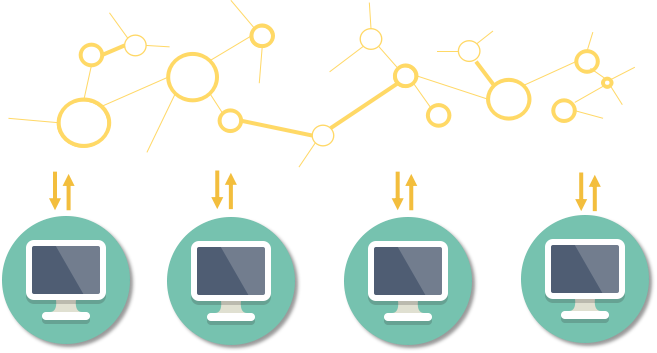
\includegraphics[width=0.8\linewidth]{multiparty.png}
\caption{Multiparty Data Exchange.}
\end{figure}
Multiple parties observing correlated data seek to recover each other's data. How can they accomplish this using minimum communication?
\begin{itemize}
\item In practice, algorithms like r-sync are used for data exchange.
\begin{itemize}
\item Uses \emph{one} guess.
\item Does not exploit the correlation between the data.
\item Needs more communication.
\item Fast and low complexity.
\end{itemize}
\item In theory, Slepian-Wolf compression is the optimal solution.
\end{itemize}

\end{block}


%----------------------------------------------------------------------------------------
%	Implementation of Slepian wolf
%----------------------------------------------------------------------------------------

\begin{block}{Implementation of Slepian-Wolf Compression }

\begin{columns} % Subdivide the first main column
\begin{column}{.5\textwidth} % The first subdivided column within the first main column
\begin{itemize}
\item Difficulties in implementation of SW coding.
\begin{itemize}
\item Search is over an exponential list in decoding.
\item Knowledge of $P_{X|Y}$ required. 
\end{itemize}
\end{itemize}
\end{column}

\begin{column}{.5\textwidth} % The second subdivided column within the first main column
\centering
\begin{figure}
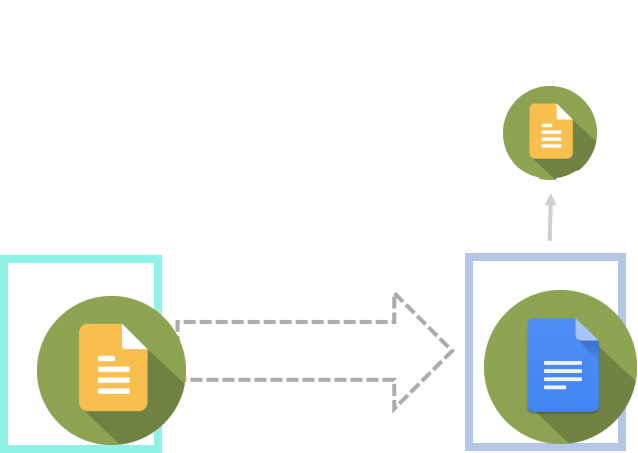
\includegraphics[width=0.9\linewidth]{slepian.png}
\caption{Slepian-Wolf Compression.}
\end{figure}
\end{column}
\end{columns} % End of the subdivision

\begin{itemize}
\item Suggested approach.
\begin{itemize}
\item Use of structured channel codes, in particular \emph{Polar codes}, for implementation of SW compression \cite{PCSW}.
\item Achieve universality using a \emph{Recursive Data Exchange protocol} (RDE)   
 \cite{HTRDE}.
\item Realise the RDE using H-ARQ based on polar codes. 
\end{itemize}
\end{itemize}

\end{block}
%----------------------------------------------------------------------------------------
%	Polar codes 
%----------------------------------------------------------------------------------------

\begin{block}{Polar Codes for Data Exchange}
\vspace{0.5cm}
\begin{columns} % Subdivide the first main column
\begin{column}{.5\textwidth} % The first subdivided column within the first main column

\begin{itemize}
\item Polar Codes for error control.
\begin{itemize}
\item N indentical and independent channels W are converted to a second set of channels which have probility of error either 0 or 1.
\item Low complexity.
\end{itemize}
\end{itemize}
\end{column}

\begin{column}{.43\textwidth} % The second subdivided column within the first main column
\centering
\begin{figure}
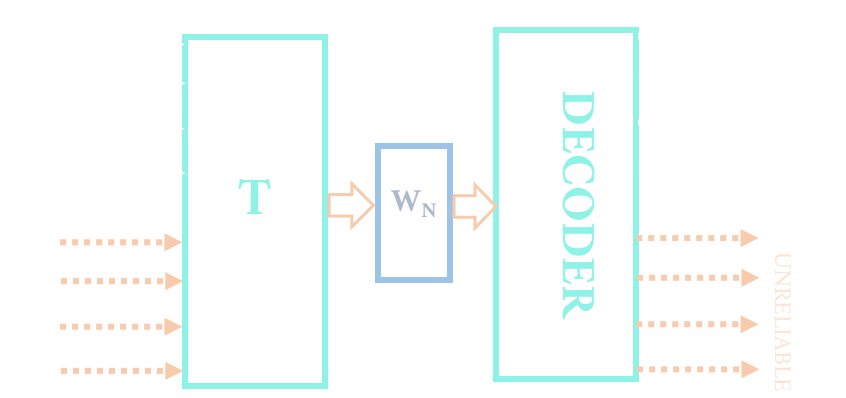
\includegraphics[width=1\linewidth]{pch.png}
\caption{Polar Coding.}
\end{figure}
\end{column}
\end{columns} % End of the subdivision

\begin{itemize}
\item Polar Codes for SW Compression.
\begin{figure}
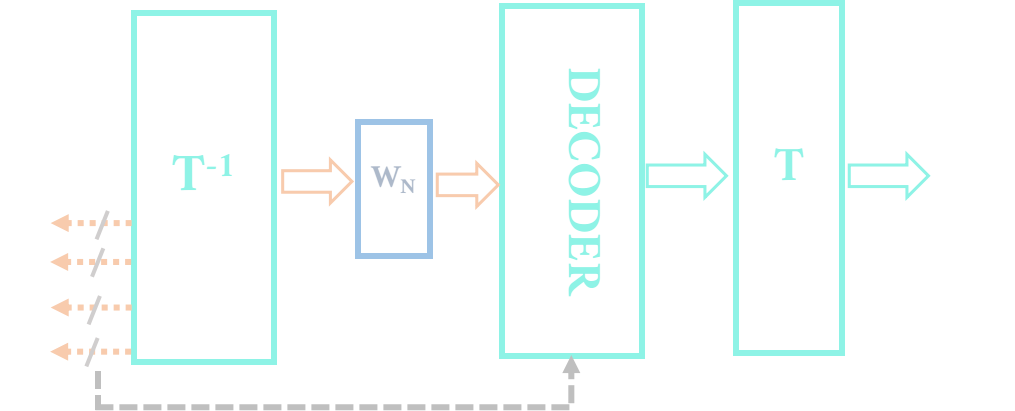
\includegraphics[width=0.7\linewidth]{psw.png}
\caption{Polar Coding for SW Compression.}
\end{figure}
\begin{itemize}
\item Here, $X_{N}$ and $Y_{N}$ are correlated. The bits that are to be sent for estimation of $X_{N}$ from $Y_{N}$ are decided by inverse Arikan transform, '$T^{-1}$', and are communicated error-free.
\end{itemize}
\end{itemize}

\end{block}

%----------------------------------------------------------------------------------------

\end{column} % End of the first column

\begin{column}{.03\textwidth}\end{column} % Empty spacer column
 
\begin{column}{.465\textwidth} % The second column

%----------------------------------------------------------------------------------------
%	OBJECTIVES
%----------------------------------------------------------------------------------------
            
%\begin{block}{Objectives}
%\begin{itemize}
%\item In practice , algorithms like \textbf{r-sync} are used for data exchange.
%\item In theory,\textbf{\emph{Slepian-Wolf compression}},is the optimal solution.
%\end{itemize}
%\end{block}

%----------------------------------------------------------------------------------------
%	RECURSIVE DATA EXCHANGE
%----------------------------------------------------------------------------------------
            
\begin{block}{Iterative SW Compression using Incremental Freezing }
\begin{itemize}
\item The RDE scheme iteratively communicates in steps until the data exchange is completed. This can be practically implemented by Hybrid ARQ.
\item In H-ARQ, initially \emph{MSG+ Error Detection Code} is sent to receiver. On unsuccessful recovery, \emph{Error Correction Code (FEC)} is communicated incrementally. 
\end{itemize}

\begin{columns} % Subdivide the first main column
 % The first subdivided column within the first main column
\begin{column}{.5\textwidth}
\begin{itemize}
\item Adaptation of H-ARQ for RDE.
\begin{itemize}
\item In Incremental Freezing, unreliable channels are chosen and information present in these channels are commmunicated \cite{KC} incrementally.
\item Error detection using CRC is not feasible in SW compression.Hence a PHY layer error detection scheme is proposed.
\end{itemize}
\end{itemize}
\end{column}
\begin{column}{.5\textwidth}
\begin{figure}
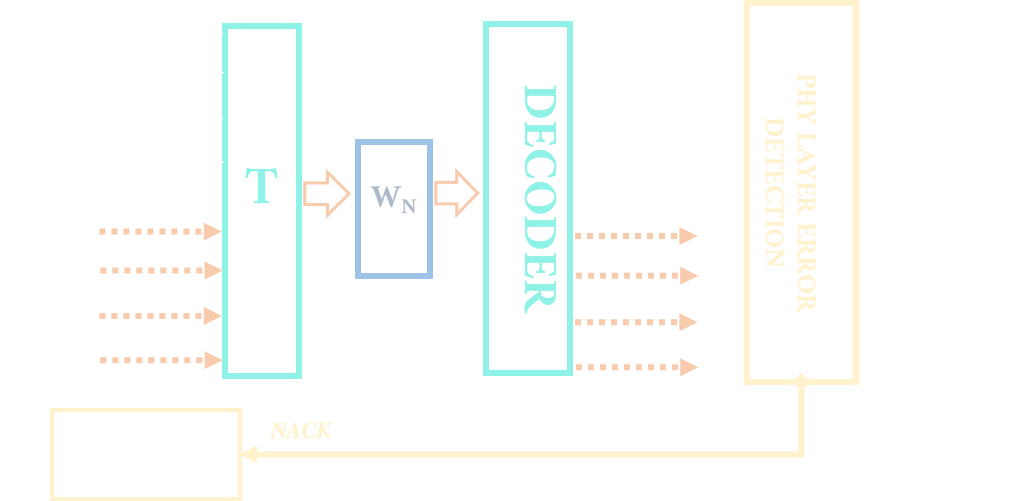
\includegraphics[width=1.1\linewidth]{PHYHARQ.png}
\caption{H-ARQ for RDE.}
\end{figure}
\end{column}
\end{columns}
\begin{columns}
\begin{column}{.5\textwidth}
\begin{itemize}
\item PHY layer Error Detection for Incremental freezing.
\begin{itemize}
\item Incremental freezing initiates assuming a high reliability channel.
\item Log-Likehood Ratios (LLR) of the bit-channels are compared to a threshold.
\item In a successful transmission a high percentage of the LLRs clear the threshold with high probability.
\item Otherwise more unreliable bits are frozen.
\end{itemize}
\end{itemize}
\end{column}
\begin{column}{.5\textwidth}
\begin{figure}
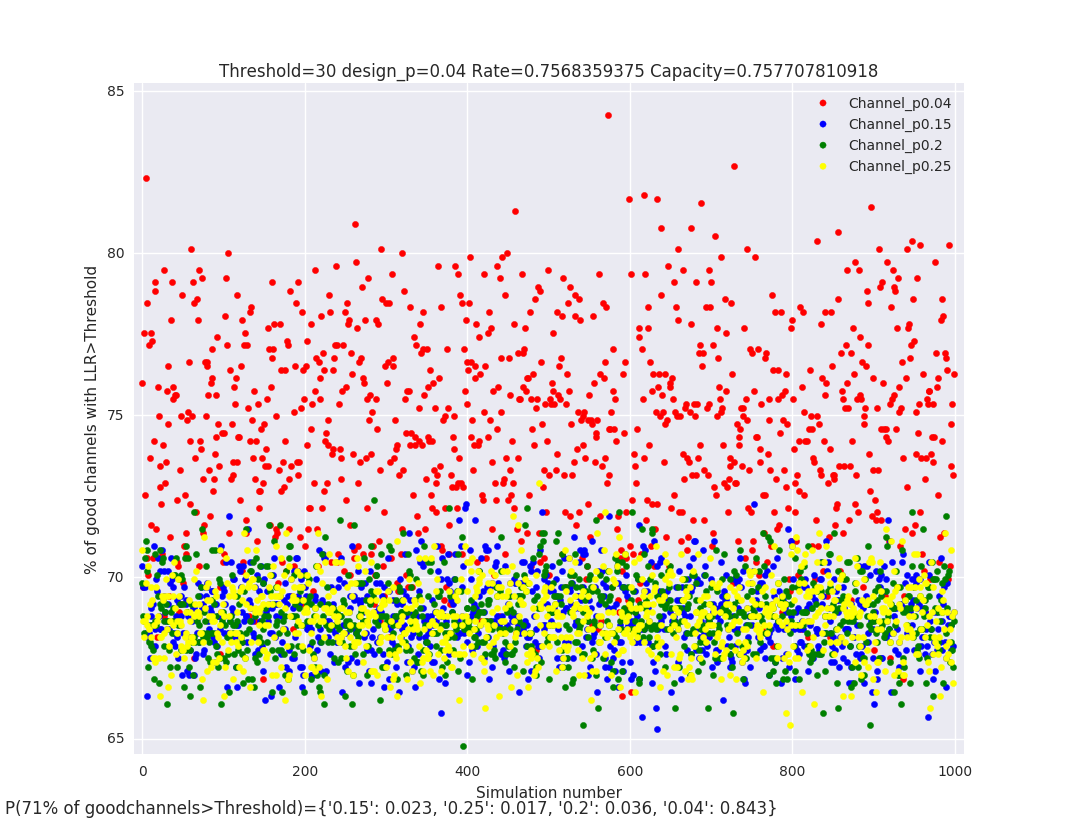
\includegraphics[width=0.9\linewidth]{theta-0p4.png}
\caption{Choice of threshold for BSC.}
\end{figure}
\end{column}
\end{columns}
\end{block}

%----------------------------------------------------------------------------------------
%	RESULTS
%----------------------------------------------------------------------------------------

\begin{block}{Results}
\begin{columns} % Subdivide the first main column
 % The first subdivided column within the first main column
%PLOT 1
\begin{column}{.5\textwidth}
\begin{figure}
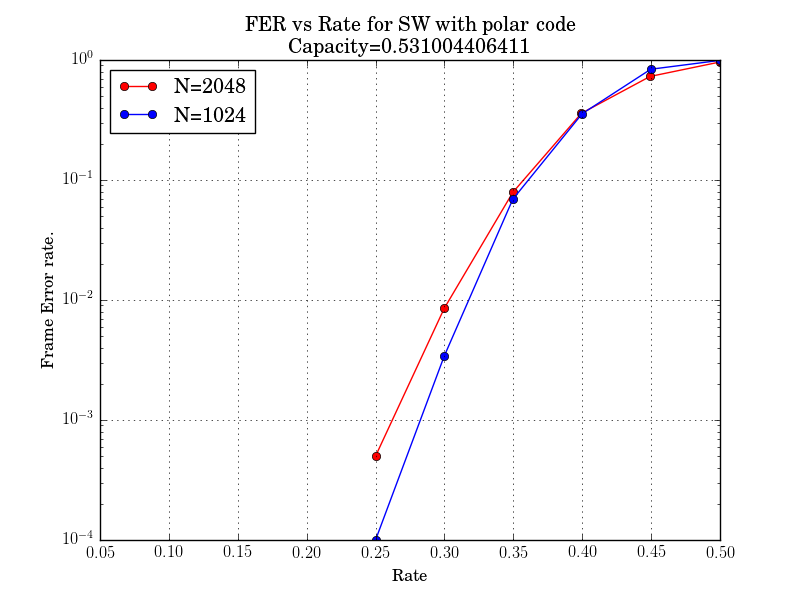
\includegraphics[width=0.9\linewidth]{swfer.png}
\caption{FER for SW compression.}
\end{figure}
\end{column}
%PLOT 2
\begin{column}{.5\textwidth}
\begin{figure}
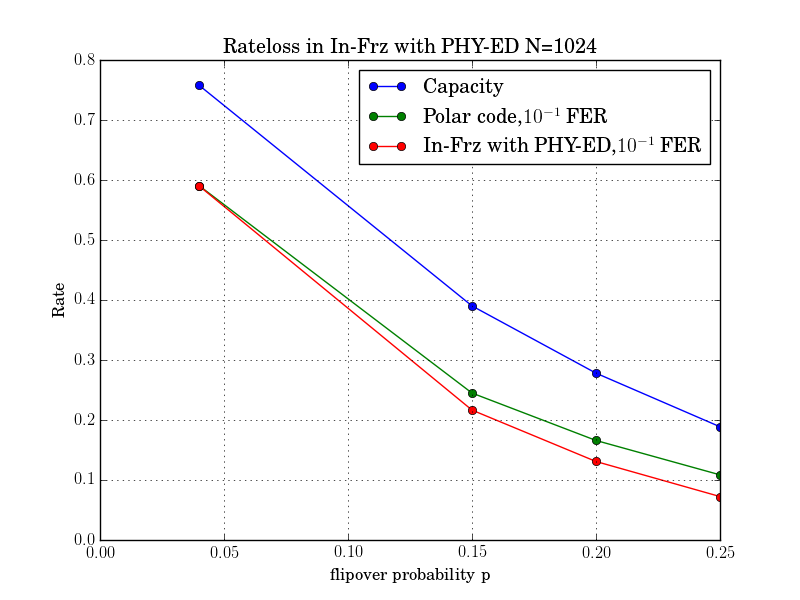
\includegraphics[width=0.9\linewidth]{rateloss.png}
\caption{Rateloss for BSC.}
\end{figure}
\end{column}
\end{columns}
\end{block}

%----------------------------------------------------------------------------------------
%	CONCLUSION
%----------------------------------------------------------------------------------------
%\setbeamercolor{block title}{fg=black,bg=orange!70}
\begin{block}{Conclusion and future work}
\begin{itemize}
\color{tacream}
\item The proposed scheme reduces communication among nodes.
\item The CRC-free universal polar code promises considerable rate gain for communication using short packet lengths.
\end{itemize}
\begin{itemize}
\item Future work.
\begin{itemize}
\item Extensive performance analysis and theoritical analysis of proposed error detection scheme as a RB-HARQ for polar codes.
\item Implementation of the scheme for multiparty data exchange.
\end{itemize}
\end{itemize}
%\color{tacream}$$\frac{1}{K_{ITER}}\sum_{i=1}^{K_{ITER}} \mathbbm{1} _{\{|LLR|_i>%\lambda_{ITER}\}} > \Theta_{ITER}$$
\end{block}

%----------------------------------------------------------------------------------------
%	REFERENCES
%----------------------------------------------------------------------------------------
\begin{block}{References}
        
\nocite{*} % Insert publications even if they are not cited in the poster
\small{\bibliographystyle{unsrt}
\bibliography{conference_poster_2}

}
\end{block}
%----------------------------------------------------------------------------------------
%	CONTACT
%----------------------------------------------------------------------------------------
\setbeamercolor{block title}{fg=black,bg=orange!70}
\begin{block}{Contact information: \textless htyagi,bsoumya\textgreater @iisc.ac.in}

%Email:bsoumya@iisc.ac.in        
\end{block}
%----------------------------------------------------------------------------------------

\end{column} % End of the second column

\begin{column}{.015\textwidth}\end{column} % Empty spacer column

\end{columns} % End of all the columns in the poster

\end{frame} % End of the enclosing frame

\end{document}
